\documentclass{mcmthesis}
\mcmsetup{CTeX = false,    % 使用 CTeX 套装时,设置为 true
          tcn = {2407108}, problem = \textcolor{red}{C},
          sheet = true, titleinsheet = true, keywordsinsheet = true,
          titlepage = false, abstract = false}
        
\usepackage{newtxtext}     % \usepackage{palatino}
\usepackage[style=apa,backend=biber]{biblatex}
\addbibresource{reference.bib}

\usepackage{tocloft}
\usepackage{subcaption}

\usepackage{float}  %控制图片和表格的位置
\usepackage{indentfirst} %s首行缩进
\usepackage{threeparttable} %添加表格注释
\setlength{\cftbeforesecskip}{6pt}
%\setlength{\parindent}{2em} %全局首行缩进2字符
\renewcommand{\contentsname}{\hspace*{\fill}\Large\bfseries Contents \hspace*{\fill}}

\title{{\bf Quantifying momentum, grasping victory in tennis}}
% \author{\small \href{http://www.latexstudio.net/}
%   {
\includegraphics[width=7cm]{mcmthesis-logo}}}
\date{\today}

\begin{document}
%%%%%%%%%%%%%%%%%%%%%%%%%%%%%%%%%%%%%%%摘要%%%%%%%%%%%%%%%%%%%%%%%%%%%%%%%%%%%%%%%%
\begin{abstract}

    Physics defines where momentum as “the strength or force gained by motion or by a series of
    events that keeps an objective moving.” In tennis, it is the psychological and physical effects of
    momentum that determine the direction of a match. The aim of this study is to {\bf investigate the
    impact of momentum in tennis matches through a data-driven approach, and to develop a
    model to predict changes in momentum in matches.} Using the Wimbledon 2023 men's singles
    tournament as a case study, we analyzed match data to quantify momentum in matches and assess
    its impact on match outcomes.\par
     {\bf Firstly}, we defined a series of momentum metrics based on factors such as “score, aces, and
    double faults”. Using these metrics, we utilized the {\bf Random Forests Algorithm} to develop a
    dynamic model capable of tracking and evaluating a player's performance during a match in real
    time. The model takes into account the higher probability of the {\bf serving team winning points} in a
    tennis match, weights the momentum score, and visualizes the flow of the match.\par
    Secondly, with respect to the role of momentum, our model challenges the conventional
    wisdom that the effect of momentum on the outcome of a match is random. To this end, we
    designed a model that reflects the percentage of players' momentum and used a {\bf logistic regression
    model} to make predictions. Some new factors were defined to quantify momentum, which
    referred to {\bf “service score rate, break failure rate, net scoring rate and so on”}, proving that
    momentum can indeed predict the outcome of a match, and that the accuracy of our model can
    reach up to {\bf 90\% and more.} \par
     {\bf Thirdly}, inspired by the {\bf Sliding Window Algorithm}, we designed a new quantitative model
    for momentum and examined its effectiveness in predicting match outcomes. We then utilized the
    use of historical data to identify key factors that lead to changes in momentum and predict shifts in
    momentum in future games. We also proposed some model-based advice for players going into a
    new match accordingly. After testing, our model can predict momentum shifts with a success rate
    of 71\% percent.\par
     {\bf Finally}, we applied the model to data from other games to test the model's ability to
    generalize. Although the model performed poorly in some cases, this prompted us to identify and
    suggest additional factors that may need to be included in future models, such as the {\bf physical
    condition of the players, weather conditions}, as well as {\bf psychological stress}. \par
    Through this study, we have provided coaches and players with data-based insights to better
    understand and apply momentum shifts in matches, providing them with strategic advice going
    into new matches. The results of our study are not only applicable in tennis, but also informative
    for other sports that require an understanding of dynamic competitive states.
\begin{keywords}
    Momentum Analysis; Predictive Modeling; Random Forest; Sliding Window; Logistic Regression;
    Data Visualization; Generalization Capability
\end{keywords}
\end{abstract}


%%%%%%%%%%%%%%%%%%%%%%%%%%%%%%%%%%%%%%%目录%%%%%%%%%%%%%%%%%%%%%%%%%%%%%%%%%%%%%%%%
\maketitle

\tableofcontents
\thispagestyle{empty}

\newpage
%%%%%%%%%%%%%%%%%%%%%%%%%%%%%%%%%%%%%%%引言%%%%%%%%%%%%%%%%%%%%%%%%%%%%%%%%%%%%%%%%
\section{Introduction}

\subsection{Background}%%%%%%%%背景
“Tennis more than any other sport, is a game of momentum. The absence of a clock to do the dirty
work of finishing off an opponent, and a scoring system based on units used, makes the flow of the
match much more important than any lead that has been established."

\hfill——Chuck Kriese

Physics defines where momentum as “the strength or force gained by motion or by a series of events that keeps an objective moving.” \cite{1} In tennis, it is the psychological and physical effects
of momentum that determine the direction of a match. A player seemingly in the ascendancy
during a match is often said to “have the momentum”. Momentum in tennis can swing wildly from
point to point, game to game, set to set. Swings in momentum are referred to as turning points. These can be obvious: players switching tactics after losing a set; a brilliant winner went on the
ropes in a rally or an untimely double fault causing a opponent tightening up.

 However, sometimes momentum can be so small as to be imperceptible, it is difficult to
measure and it is not readily apparent how various events during the match act to create or change
momentum if it exists. By understanding and tapping momentum, players can employ methods
and tactics in games to ensure they are in control of momentum rather than a victim of it.

\subsection{Restatement of the Problem}%%%%%%%%问题重述
Through in-depth analysis and research on the background of the problem, combined with
topic specific constraints and requirements given, the restate of the problem can be expressed as
follows: 
\begin{itemize}
    \item {\bf Construct a model to capture the flow of play as points occur.} Identifying which player
    is performing better at a given time in the match, as well as how better they are performing. A
    visualization based on the model is required to depict the match flow. It is also noteworthy
    that the player to serve are supposed to be factored in to the model. 
    \item {\bf Use the model to assess whether “momentum” plays any role in a match}, as well as
    swings in play and runs of success by one player are random. 
    \item {\bf Identify indicators of the changing flow of play from favoring one player to the other.} Use the data provided to develop a model that predicts these swings in the match and try to
    probe into the most related factors. Advise a player going into a new match against a
    different player with the differential in past match “momentum” swings.
    \item {\bf Test the developed model on other matches and identify factors that might need to be
    added.}
    \item {\bf Produce a report of no more than 25 pages with the above findings and include a one-to two-page memo}, summarizing the results with advice for coaches on the role of “momentum”, and how to prepare players to respond to events that impact the flow of play
    during a tennis match.
\end{itemize}

\subsection{Our Work}%%%%%%%%文章分析

\begin{figure}[H]
    \centering
    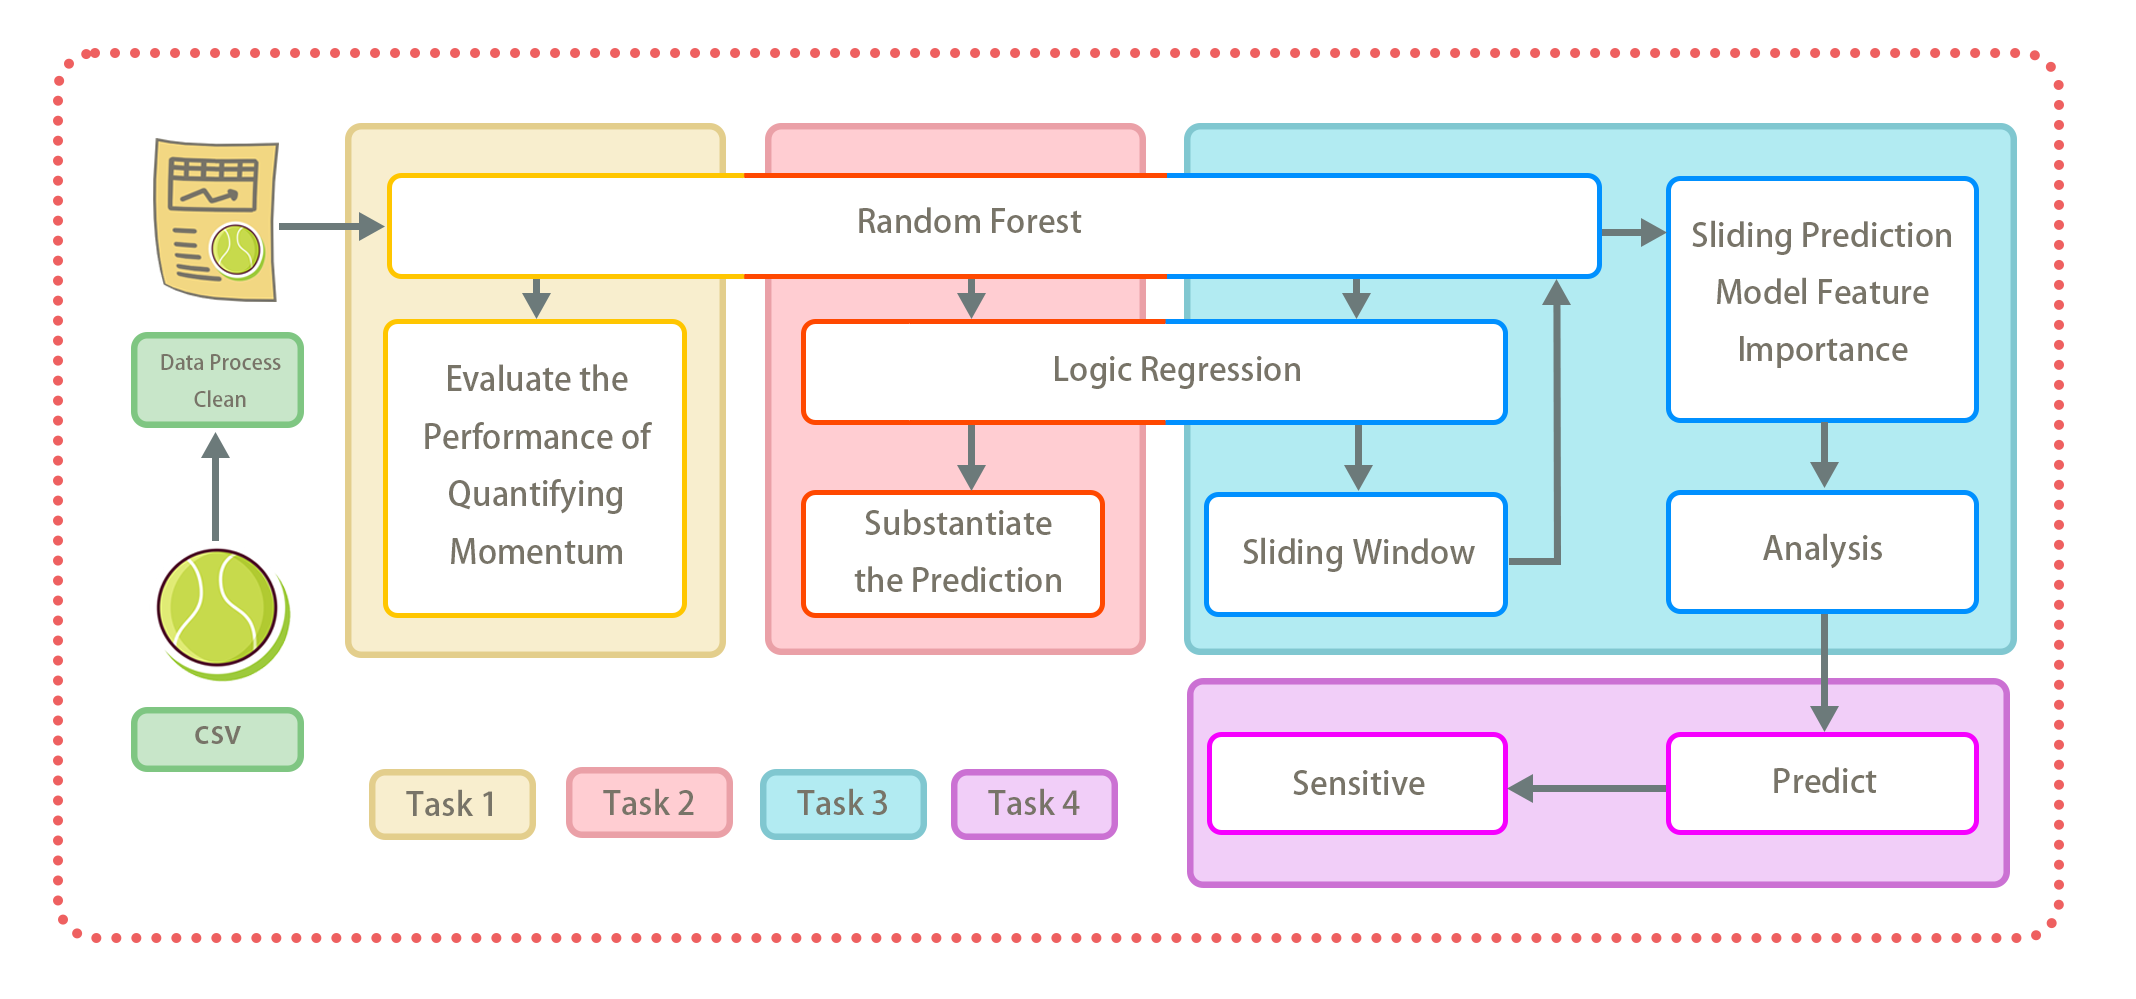
\includegraphics[width=12cm]{process.png}
    \caption{Modeling process} 
\end{figure}
%%%%%%%%%%%%%%%%%%%%%%%%%%%%%%%%%%%%%%%假设%%%%%%%%%%%%%%%%%%%%%%%%%%%%%%%%%%%%%%%%
\section{Assumptions and Justification}
\begin{itemize}

    \item {\bf Athletes will not be affected by the results of previous matches while playing the
    current match.} Supposing that the athlete is always in a good state of mind and that his or her
    performance in the previous game does not affect the outcome of the current game. 
    
    \item {\bf Athletes have a fixed interval between each score.} Supposing the interval between goals
    can be equated to the concept of time. In this way the time cost of scoring is quantifiable and
    relatively stable in the tennis match and we can analyze game progression and athletes' performance from a new perspective.

\end{itemize}
%%%%%%%%%%%%%%%%%%%%%%%%%%%%%%%%%%%%%%%符号说明%%%%%%%%%%%%%%%%%%%%%%%%%%%%%%%%%%%%%%%%
\section{Notations}
Table 1 shows the necessary notations and signs used in this paper. Other notations and signs
will be declared or defined when using.\cite{[2]}

\begin{table}[H]
    \centering
    \renewcommand{\arraystretch}{1} % 调整行间距
    \caption{\textbf{Notations}} % 加粗标题
    \vspace{0.5em} % 增加标题与表格之间的距离
    \begin{tabularx}{\textwidth}{ll}
    \toprule[2pt]
    \textbf{Symbols} & \textbf{Descriptions} \\ 
    \midrule[1pt]
    $S_{P1i}$ & player 1's momentum integral value in one match \\ 
    $S_{P2i}$ & player 2's momentum integral value in one match \\ 
    $A_r$ & service score rate \\ 
    $F_r$ & service failure rate \\ 
    $B_r$ & break success rate \\ 
    $B_f$ & break failure rate \\ 
    $N_r$ & net scoring rate \\ 
    $E_r$ & error ratio \\ 
    $T_S$ & the total number of serve in the set \\ 
    $M$ & momentum \\ 
    \bottomrule[2pt]
    \end{tabularx}
    \label{Table:Notations}
\end{table}

%%%%%%%%%%%%%%%%%%%%%%%%%%%%%%%%%%%%%%%数据处理%%%%%%%%%%%%%%%%%%%%%%%%%%%%%%%%%%%%%%%%
\section{Data Preprocessing} 

\subsection{Data Cleaning}

{\bf Overview of data sets:} This dataset is derived from the featured races of the Wimbledon Championship and contains detailed race statistics.
 It is worth noting that there are a number of missing values in the dataset, particularly in the speed\_mph (752 missing), serve\_width and
serve\_depth (54 missing each), and return\_depth (1309 missing) fields. 

{\bf Missing value handling: }In dealing with missing values in the dataset, special attention is
paid to the NA values in the speed column. In an initial check, 752 missing values were found in
the speed column. These missing values can occur for a variety of reasons, including data entry
errors or omissions during the data collection process. There were even instances in matches 1310
and 1311 where the whole bureau had unrecorded rally\_count as well as speed values. 

Further analysis showed that some of the missing speed values were associated with a
rally\_count of 0, which reflected a specific scenario of a no-ball exchange during the match, not
missing data, as shown in \ref{Figure 1}. In contrast, the missing data for complete matches may stem
from technical problems or human negligence in the recording process.

\begin{figure}[htbp]
    \centering
    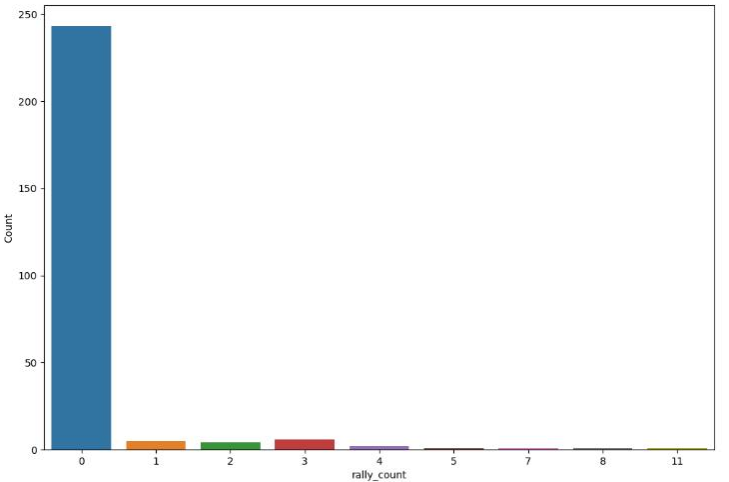
\includegraphics[width=12cm]{screencut 2025-01-22 142335.png}
    \caption{SpeedNA\_Count\_By\_RallyCount} \label{Figure 1}
\end{figure}


In the case of unrecorded data for an entire race, we decided to exclude these records from
the dataset given the non-direct impact of this data on model training. Data where a rally\_count of
0 resulted in a speed of 0 was considered a valid record and retained to accurately reflect the
reality of the race. 

Through this careful missing value handling strategy, we ensured the accuracy and reliability
of the data analysis and laid a solid foundation for the subsequent data analysis work. 

{\bf Abnormal value progress:} In the dataset, there are 235 rows of records showing that when
double fault is 1, the serve\_width and serve\_depth fields are still recorded. Theoretically, in the
event of a double serve fault, the ball did not successfully cross the net and therefore the width and
depth of the serve should not be recorded.

\subsection{Data Analysis}
We find that serve\_no and speed are related. The box plot shows the distribution of serve
speeds according to the number of serves (first and second). The following points can be observed
from the graph:

\begin{figure}[htbp]
    \centering
    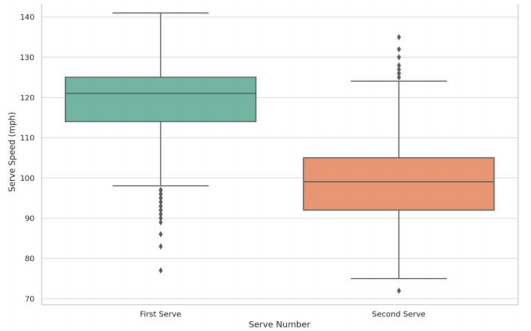
\includegraphics[width=12cm]{screencut 2025-01-22 142718.png}
    \caption{Boxplot of Serve Speed By Serve Number} \label{Figure 2}
\end{figure}

First serve speeds were typically higher than second serve speeds, reflecting a common
strategy in tennis whereby players tend to use more powerful serves on the first serve in an
attempt to score points outright or to gain a favorable position, while they tend to use more secure
serves on the second serve to avoid double faults.

The wider distribution of speeds on the first serve and the higher outliers at the top suggest
that players' serve speeds vary more when attempting more powerful serves. 

The relatively more concentrated distribution of speeds and fewer outliers on the second
serve may be due to the fact that players focus more on accuracy and consistency on the second
serve to minimize the risk of double faults. 

These observations are consistent with the conventional strategy in tennis where the first
serve is more focused on aggressiveness while the second serve is more focused on insurance. This analysis helps us to gain a deeper understanding of players' serving strategies and their
potential impact on match outcomes.

%%%%%%%%%%%%%%%%%%%%%%%%%%%%%%%%%%%%%%%模型结构%%%%%%%%%%%%%%%%%%%%%%%%%%%%%%%%%%%%%%%%
\section{Model Construction}

\subsection{Discrete Performance Evaluating Model Based on Random Forest} %%%%基于随机森林的离散性能评价模型

\subsubsection{Model Preparation} %%%%%%%%%%%%%%模型准备

According to the requirements of problem 1, this paper needs to build a model to obtain the
scoring points occurring in the match. {\bf The Random Forest model} is chosen to determine the
weights of the indicators, therefore we are able to identify the better performance of the players
visually, then we apply the model to as many games as possible.

\begin{itemize}
    \item {\bf Firstly, we acquire data information such as “ace” or “net\_pt” }, which refer to a not- served shot and a player’s position separately from the provided data set, result data of each set
    or game can also be found.
    \item {\bf Next, we try to design a model to quantify “momentum”.} Momentum can be perceived as
    strength or force during a match, since it is difficult to quantize, so we attempt to incorporate the
    Calculation of short-term indicators, transforming scoring concepts into momentum indicators. 
    \item {\bf Then, we discover that momentum is usually reflected as a change in game
    performance over a short period of time. }For example, consecutive scores can be seen as a
    direct reflection of momentum. By calculating short-term changes in scoring for each point
    (e.g., consecutive points, short-term serve success and break rates, etc.), these short-term
    performances can be quantified as indicators of momentum.
\end{itemize}

\subsubsection{Random Forest Model}  %%%%%%%%%%%%%随机森林
Although the ultimate goal is to predict the outcome of the game, the impact of momentum
changes on the outcome of the game can be revealed by analyzing the relationship between short-term momentum indicators and the final outcome of the game. Short-term momentum indicators
can be trained as features and match results (win/lose) as labels in the model to determine the
association between momentum and match. 

We can begin to quantify indicators by virtue of the above idea, but it is not yet possible to
determine the specific levels of quantification. We then use a random forest model to analyze the
importance of the characteristics of these indicators. 

Random Forest is a supervised algorithm that uses an integrated learning method consisting
of numerous decision trees. It's able to handle large and complex datasets, including multiple
types of variables, which is useful for analyzing the impact of various factors in tennis matches. What is more, it can provide an effective method for assessing the importance of individual
features in predicting outcomes, which allows to identify which factors have the greatest impact
on player momentum and match results.\cite{[4]}

\begin{figure}[htbp]
    \centering
    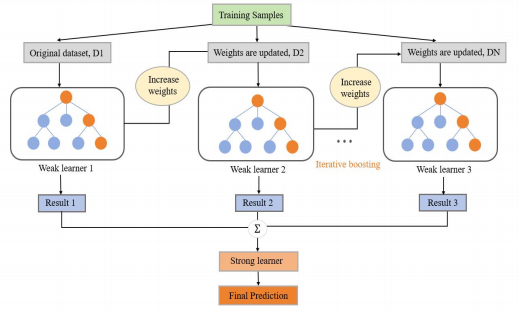
\includegraphics[width=12cm]{screencut 2025-01-22 143525.png}
    \caption{Concept of Random Forest} \label{Figure 3}
\end{figure}

Therefore we try to describe the method by means of detail principles of the Random Forest
model, including how it handles large numbers of input variables and evaluates the importance of
features. We can explain the source of the dataset, the variables chosen (e.g., score, serve success
rate, unforced errors, etc.), and how the data were prepared for use in the analysis accordingly.\\
We focus on the characteristic importance scores of each factor's impact on the outcome of
the match. Specially, we weight the “serve” artificially low.\\
The results of the Random Forest Model analysis are in the following graphs.

\begin{table}[H]
    \centering
    \caption{\textbf{Feature Importance Ranking in Random Forest Model}}
    \vspace{0.5em}
    \begin{tabularx}{\textwidth}{>{\centering\arraybackslash}X>{\centering\arraybackslash}X>{\centering\arraybackslash}X}
    \toprule[2pt]
    \textbf{Order} & \textbf{Features}     & \textbf{Weights} \\ 
    \midrule[1pt]
    1              & break\_pt             & 0.275942         \\ 
    2              & point\_victor         & 0.168837         \\ 
    3              & unf\_err              & 0.139420         \\ 
    4              & winner                & 0.108685         \\ 
    5              & ace                   & 0.095252         \\ 
    6              & double\_fault         & 0.077130         \\ 
    7              & net\_pt               & 0.074068         \\ 
    8              & net\_pt\_won          & 0.039238         \\ 
    9              & break\_pt\_missed     & 0.021428         \\ 
    \bottomrule[2pt]
    \end{tabularx}
    \label{tab:feature_importance}
    \end{table}
    

\begin{figure}[htbp]
    \centering
    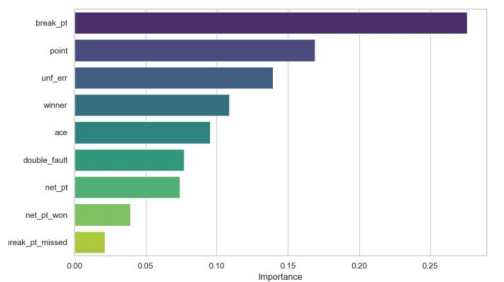
\includegraphics[width=12cm]{screencut 2025-01-22 143838.png}
    \caption{Feature Importance in Random Forest Model} \label{Figure 4}
\end{figure}

According to the chart presented above, we define the following weights:

\begin{equation} \label{(1)}
    \begin{split}
      W &= (0.275942, 0.8 \times 0.168837, -0.139420, 0.108685, \\
      &\quad -0.095252, 0.077130, 0.074068, 0.074068, -0.021428)
    \end{split}
\end{equation}
    

\begin{equation} \label{(2)}
    M= \sum_{n=1}^{9} W_{i}\times \alpha_{i}  
\end{equation}
%%%%%%%%%%%%%%%%%%%%%%%%%%%%%%%%%%%%二张图片%%%%%%%%%%%%%%%%%%%%%%%%%%%%%%%%%%%%
\begin{figure}[htbp]
    \centering
    \begin{subfigure}{0.45\textwidth}
        \centering
        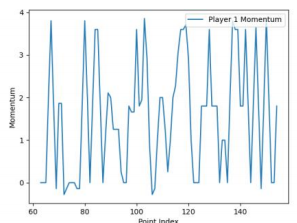
\includegraphics[width=\textwidth]{screencut 2025-01-22 145607.png}
        \caption{Player 1's Momentum}
        \label{subfig:player1}
    \end{subfigure}
    \hfill
    \begin{subfigure}{0.45\textwidth}
        \centering
        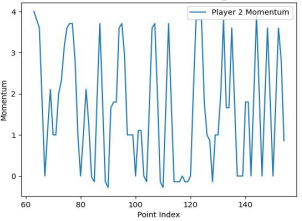
\includegraphics[width=\textwidth]{screencut 2025-01-22 145612.png}
        \caption{Player 2's Momentum}
        \label{subfig:player2}
    \end{subfigure}
    \caption{Player 1/2's Momentum in this set}
    \label{Figure6-7}
\end{figure}
%%%%%%%%%%%%%%%%%%%%%%%%%%%%%%%%%%%%二张图片%%%%%%%%%%%%%%%%%%%%%%%%%%%%%%%%%%%%
\begin{figure}[htbp]
    \centering
    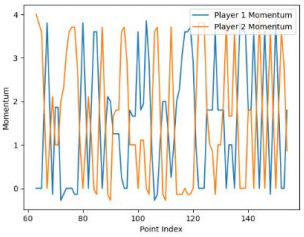
\includegraphics[width=8cm]{screencut 2025-01-22 145616.png}
    \caption{Player 1's vs Player 2's Momentum Comparison in the set\_no} \label{Figure 6}
\end{figure}

This picture above reflects the fact that the momentum values of the two players are in a state
of waxing and waning, which basically corresponds with players' actual state in a real game.\cite{3}

\begin{figure}[htbp]
    \centering
    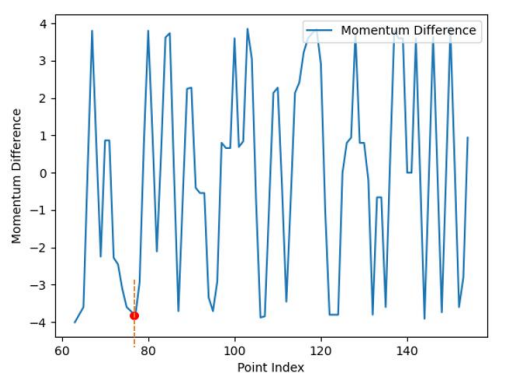
\includegraphics[width=8cm]{D:/github/MCM/test/kacey/picture/150626.png}
    \caption{Player 1-Player's Momentum Difference Comparison in this set\_no} \label{Figure 7}
\end{figure}

This picture above shows that in which time period which athlete performs better. For
example, the red spot in the diagram indicates that at the 78-minute mark of the opening, Player
1's momentum minus player 2's momentum is negative, which represents clearly that at this time, player 2 performs better than player 1.


%%%%%%%%%%%%%%%%%%%%%%%%%%%%%%%%%%%%四张图片%%%%%%%%%%%%%%%%%%%%%%%%%%%%%%%%%%%%
\begin{figure}[htbp]
    \centering
    % 减少顶部间距
    \vspace{-0.15in}
    
    % 第一行两张图片
    \begin{minipage}{1\linewidth}
        \subfloat[]{\label{fig:2.1}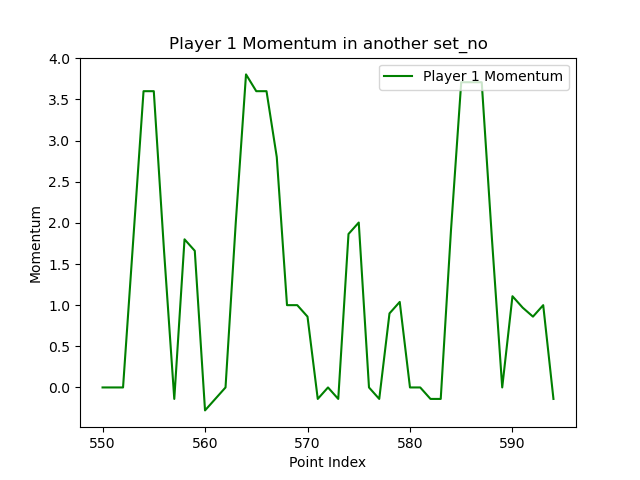
\includegraphics[width=0.45\linewidth]{2.1.png}}
        \hfill % 水平填充
        \subfloat[]{\label{fig:2.2}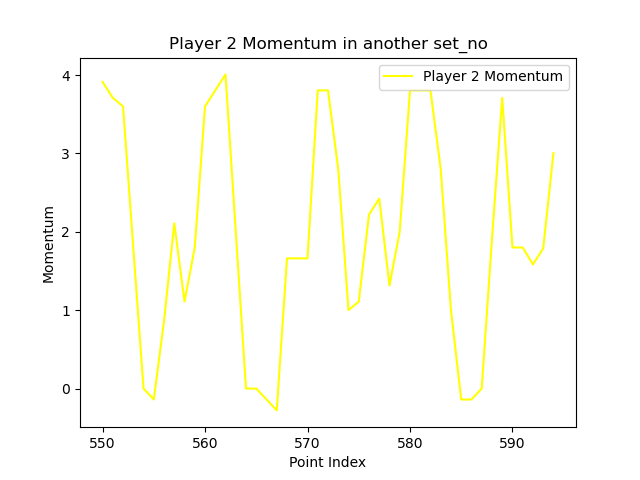
\includegraphics[width=0.45\linewidth]{2.2.png}}
    \end{minipage}
    
    % 减少两行图片之间的间距
    \vskip -0.3cm
    
    % 第二行两张图片
    \begin{minipage}{1\linewidth}
        \subfloat[]{\label{fig:2.3}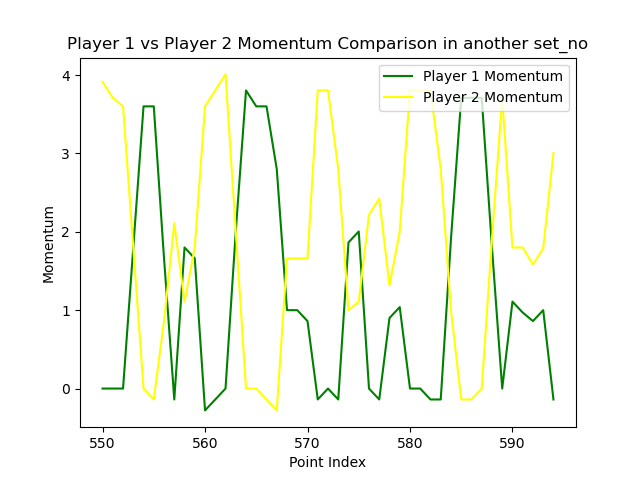
\includegraphics[width=0.45\linewidth]{2.3.png}}
        \hfill % 水平填充
        \subfloat[]{\label{fig:2.4}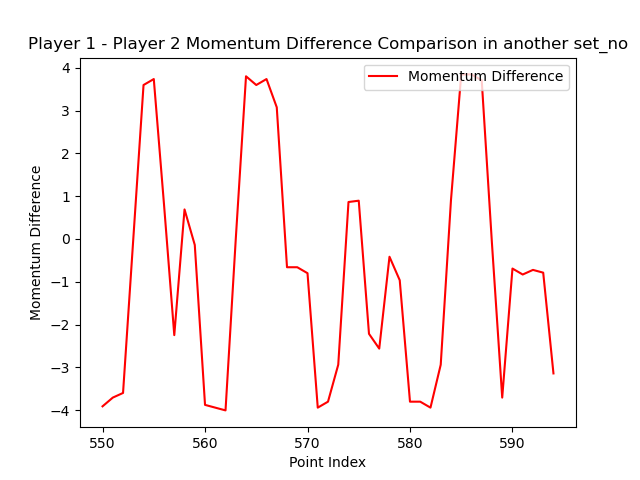
\includegraphics[width=0.45\linewidth]{2.4.png}}
    \end{minipage}
    
    % 减少底部间距
    \vspace{-0.18in}
    
    \caption{Model Application Diagram} \label{fig:8-11}
\end{figure}
%%%%%%%%%%%%%%%%%%%%%%%%%%%%%%%%%%%%四张图片%%%%%%%%%%%%%%%%%%%%%%%%%%%%%%%%%%%%



%%%%%%%%%%%%%%%%%%%%%%%%%%%%%%%%%%%%三张图片%%%%%%%%%%%%%%%%%%%%%%%%%%%%%%%%%%%%
%%\usepackage{graphicx}
%%\usepackage{subfigure}

% \begin{figure}[htbp]
% 	\centering
% 	\subfigure[Picture a title] {\includegraphics[width=.3\textwidth]{hair_dryer_cloud.png}}
% 	\subfigure[Picture b title] {\includegraphics[width=.3\textwidth]{microwave_cloud.png}}
% 	\subfigure[Picture c title] {\includegraphics[width=.3\textwidth]{pacifier_cloud.png}}
% 	\caption{Example 1 picture title}
% 	\label{fig_E1}
% \end{figure}

%%%%%%%%%%%%%%%%%%%%%%%%%%%%%%%%%%%%三张图片%%%%%%%%%%%%%%%%%%%%%%%%%%%%%%%%%%%%


\subsection{Assessment Based on Logistic Regression}

\subsubsection{Assessment Preparation}
According to the requirements of the problem, this paper needs to assess that “momentum”
actually plays an role in a match and swings in play and runs of success by one player are not
random but correlative. We choose {\bf Logistic Regression in classification algorithms} to train the
model, then we can obtain the training results with higher predicted value. Finally we are able to
visualize the description based on the model results to prove the crucial role “momentum” acts in
the match and its high relevancy.

Through the weight we determine in the previous question, we are able to derive two chart
with its horizontal axis coordinates are the number of points scored per game and the vertical axis
coordinates are the momentum values for each player. Then we integrate the momentum value
folds in the two charts separately.
\begin{figure}[H]
    \centering
    \includegraphics[width=12cm]{势.png}
    \caption{Player 1's Momentum in this set\_no} \label{Figure 12}
\end{figure}
Accordingly, we can acquire the total momentum value for each player. 

By analogy with the definition “work” in physics, we figure that momentum can also
accumulate over time, so we define three values:$S_{P1}$,$S_{P2}$,$X_{i}$

In the same way, we accordingly integral to get the cumulative value of the momentum of the
two athletes in the current match, so we build this model:
\begin{equation} \label{3}
    X_{i}=\frac{S_{p1i}}{S_{p1i}+S_{p2i}}  
\end{equation}
Since there are many rounds in the competition, the momentum performance of the athletes
will vary accordingly, so there will be multiple $X_{i}$,$Y_{i}$represents the results of the set, we stipulate
that :
\begin{equation} \label{4}
    Y_{i} = 0, P_{1} \text{ loses the set}
\end{equation}
\begin{equation} \label{5}
    Y_{i} = 1, P_{1} \text{ wins the set}
\end{equation}

So we can capture series of dataset($X_{i}$,$Y_{i}$)

Through the original data scatter plot, we notice that the distribution of $X_{i}$is quite compact, so we choose to standardize $X_{i}$to make it more discrete, as it shown in the following diagram:

\begin{figure}[H]
    \centering
    \begin{subfigure}{0.45\textwidth}
        \centering
        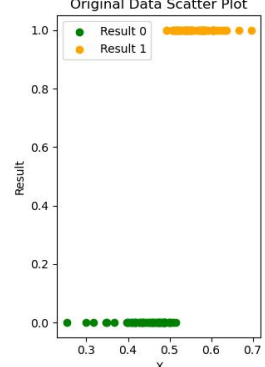
\includegraphics[width=\textwidth]{153451.png}
        \caption{Player 1's Momentum}
        \label{subfig:player1}
    \end{subfigure}
    \hfill
    \begin{subfigure}{0.45\textwidth}
        \centering
        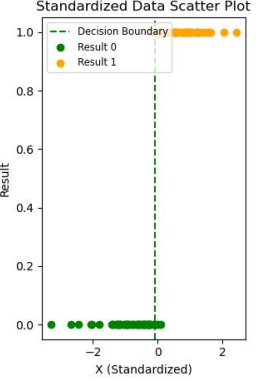
\includegraphics[width=\textwidth]{153457.png}
        \caption{Player 2's Momentum}
        \label{subfig:player2}
    \end{subfigure}
    \caption{Two Types of Data Scatter}
    \label{Figure 13}
\end{figure}

We then use {\bf Logistic Regression}:

\begin{equation} \label{6}
    \vec{w}\gets \vec{w}+\eta \sum_{i=1}^{n} \frac{y_{i}\vec{x}_{i}}{1+exp(y_{i}\vec{w}\cdot\vec{x}_{i}) }
\end{equation}

We apply the above function to approximate the optimal value. Then we take 80\% of the
dataset as training set, the rest 20\% of the dataset as test set.\cite{[5]} After the training, we can derive
the outcome. The result of the training can be shown in the following figure:

\begin{figure}[H]
    \centering
    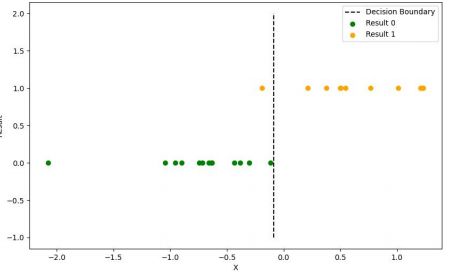
\includegraphics[width=8cm]{D:/github/MCM/test/kacey/picture/154248.png}
    \caption{Logistic Regression Decision Boundary} \label{Figure 14}
\end{figure}

We are able to observe that the predictions of the remaining test set using this method have an
{\bf rather high accuracy which even reach 90\% or more}. \\
The visualization of the accuracy rate can be seen as follows:

\begin{figure}[htbp]
    \centering
    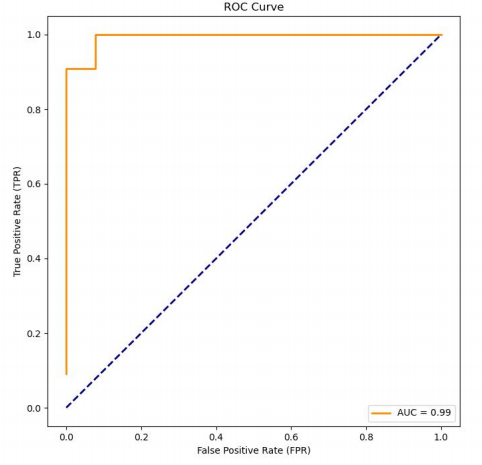
\includegraphics[width=8cm]{D:/github/MCM/test/kacey/picture/154253.png}
    \caption{ROC Curve} \label{Figure 15}
\end{figure}

The ROC Curve demonstrate that the momentum of the players in the match do show strong
correlation. The blue diagonal line represents the random situation, and the orange laddered
straight line represents the normal situation of the swings in play and runs of success by one player. Differences are distinct and convincing. {\bf Therefore, swings in play and runs of success by one
player are not random but correlative.}

\subsection{Continuous Performance Evaluating Model Based on Sliding Window}

\subsubsection{Model Preparation}
According to the requirements of the problem, this paper needs to build another model to
analyze the swings and performance of the player in one match. Given that the hypothesis of our
assumption is no longer applicable, we have to reconsider the features to make our new model
much more practical. Inspired by the {\bf Sliding Window Algorithm}, combining with the new
features or factors and new weights, we successfully construct a model and illustrate it visually. Therefore we are able to predict the swings and the flow of the match, and make preparations for
providing an useful competition suggestion.

 The previous model will not be able to solve the current problem because we did not consider
the impact of the previous game's results on the current game. Therefore, we remove the previous
assumption, and incorporate the performance and results of the previous game into the impact of
the momentum of the current game, and redefine the new indicators with corresponding new
weights to measure momentum. The redefined indicators are as follows:
\begin{equation} \label{7}
    A_{r}=\frac{Sum(ace)}{Ts}
\end{equation}
\begin{equation} \label{8}
    F_{r}=\frac{Sum(double_fault)}{Ts}
\end{equation}
\begin{equation} \label{9}
    B_{r}=\frac{Sum(break_pt_won)}{Sum(break_pt)}
\end{equation}
\begin{equation} \label{10}
    B_{fr}=\frac{Sum(break_pt_missed)}{Sum(break_pt)}
\end{equation}
\begin{equation} \label{11}
    N_{r}=\frac{Sum(net_pt_won)}{Sum(net_pt)}
\end{equation}
\begin{equation} \label{12}
    E_{r}=\frac{Sum(p2_winner)}{Sum(unf_err)}
\end{equation}

In the previous question, we only considered the single-inning case, which only involves the
accumulation of the number of points scored by a simple player as a quantitative indicator of
momentum; whereas now we need to {\bf consider the quantification of momentum within a
scoring interval, i.e., reflected by an intuitive ratio.} For example,$A_{r}$
refers to Service Score Rate, which consists of the ratio between the number of points served to the total number of serves
made in the set. Therefore, we can define other ratios such as $F_{r}$,$B_{r}$, $B_{fr}$,$N_{r}$,$E_{r}$
that presented in
the notation table. 

In addition, it's worth noting that the formation of $E_{r}$ is different. $E_{r}$ is composed of the ratio
of forced errors to unforced errors. We make a conversion to better illustrate the formula. Here, forced errors refer to the total sum of errors caused by a player failed to receive an opponent's
untouchable shot, i.e., as a numerator, forced errors are represented by the total sum of the other
player's winners in the match.

 After we define the new indicators, we apply the Random Forest algorithm to find the new
feature weights of the above feature indicators. The results are presented as follows:

\begin{table}[H]
    \centering
    \caption{\textbf{Feature Importance Ranking in Random Forest Model}}
    \vspace{-0.3pt}
    \begin{tabularx}{\textwidth}{>{\centering\arraybackslash}X>{\centering\arraybackslash}X>{\centering\arraybackslash}X}
    \toprule[2pt]
    \textbf{Order} & \textbf{Features}     & \textbf{Weights} \\ 
    \midrule[1pt]
    1              & break\_fail\_ratio    & 0.247522         \\ 
    2              & point\_victor         & 0.168837         \\ 
    3              & unf\_err              & 0.139420         \\ 
    4              & winner                & 0.108685         \\ 
    5              & ace                   & 0.095252         \\ 
    6              & double\_fault         & 0.077130         \\ 
    7              & net\_pt               & 0.074068         \\ 
    8              & net\_pt\_won          & 0.039238         \\ 
    9              & break\_pt\_missed     & 0.021428         \\ 
    \bottomrule[2pt]
    \end{tabularx}
    \label{tab:feature_importance}
    \end{table}

\begin{figure}[H]
    \centering
    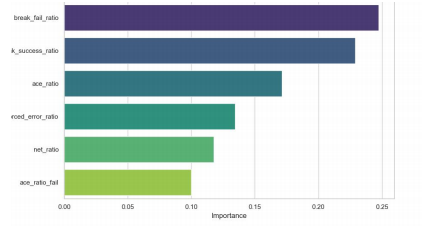
\includegraphics[width=8cm]{screencut 2025-01-22 160249.png}
    \caption{Feature Importance in Random Forest Model} \label{Figure 16}
\end{figure}

According to the chart presented above, we define the following weights:
\begin{equation} \label{13}
    \begin{split}
        W &= ( -0.247422, 0.229059, 0.139077, 0.171377, \\
        &\quad -0.134501, 0.117746, -0.099895 )
    \end{split}
\end{equation}
    

\begin{equation} \label{14}
    M=\sum_{i=1}{6}W_{i}\times\beta _{i}
\end{equation}

From this, we can further analyze the conclusions we visualized: we can see from the ranking
of the weights of the feature indicators that the breakout failure rate, who has the greatest impact
on quantifying the momentum indicators, turns out to be the most related factor among all; While
the relative breakout success rate also should not be underestimated in terms of its impact on
momentum quantification. It's in line with the reality that {\bf an athlete's success in blocking a
powerful attack against an opponent has a huge impact on his morale in subsequent matches}. What is more, the weaker impact of the net scoring rate indicator on momentum
quantification is due to the fact that players feel it risky when hitting the net, and it is more
difficult to be able to receive a baseline ball from an opponent, {\bf so players mostly do not incline
to stand in a more forward position to hit the ball}.

\begin{figure}[htbp]
    \centering
    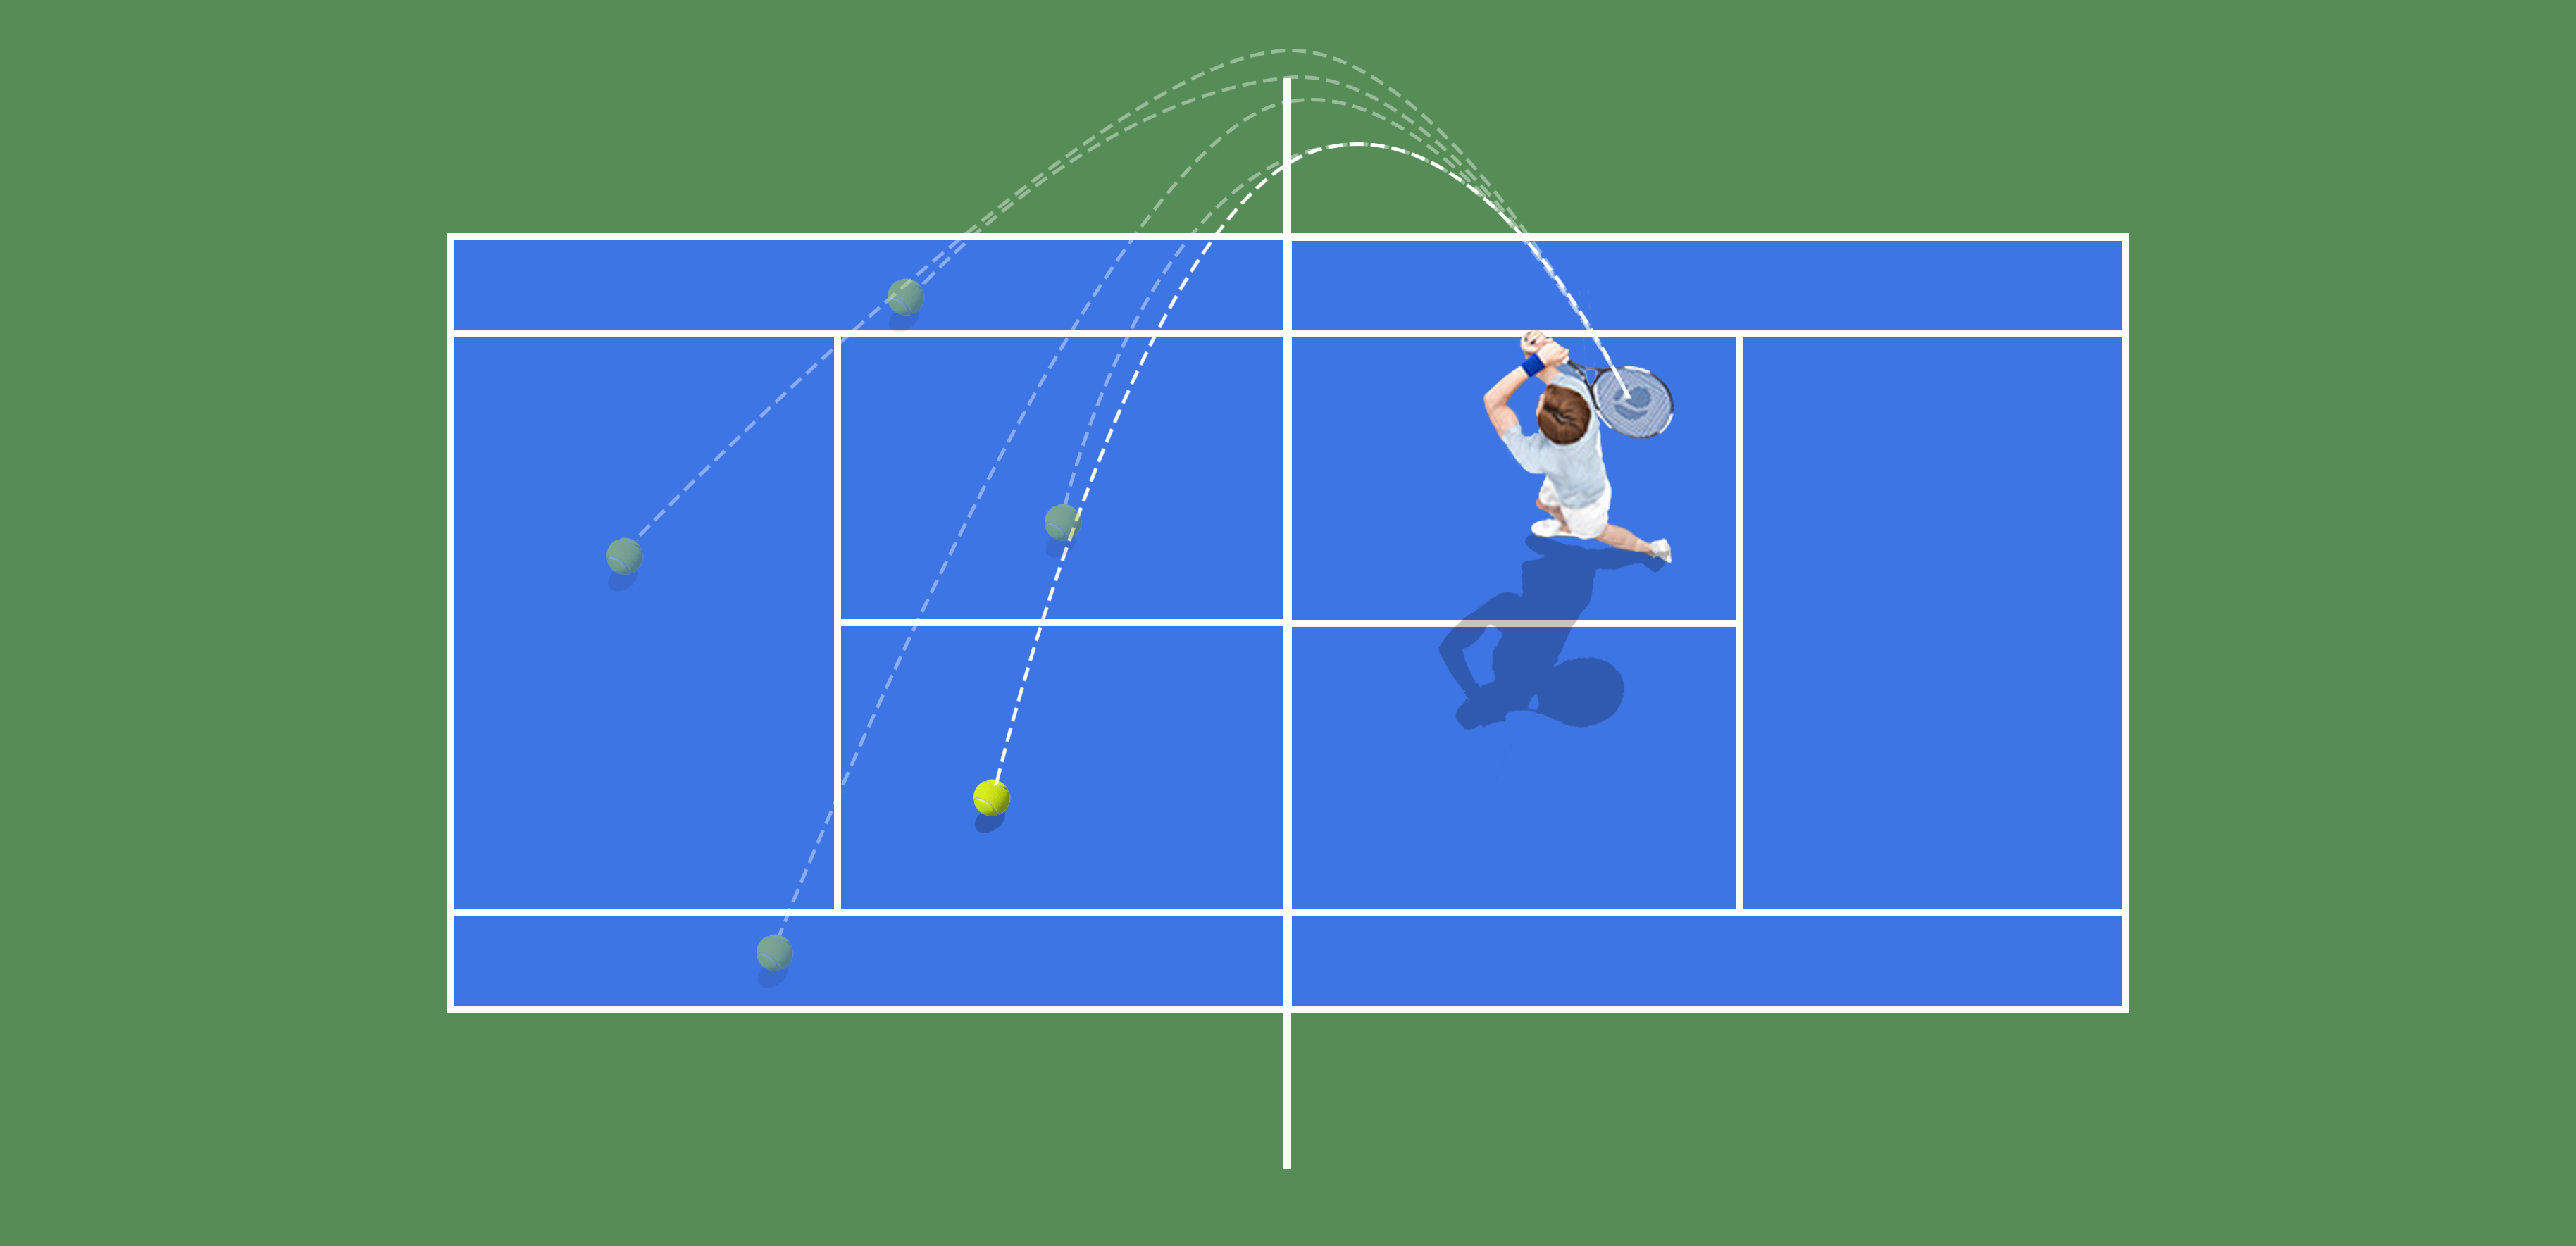
\includegraphics[width=12cm]{网球抛物线.png}
    \caption{sketch of net scoring} \label{Figure 17}
\end{figure}

Such analysis is more consistent with reality, and measurement over time can further reflect trends in momentum over time in preparation for subsequent modeling.

\subsubsection{Sliding Window Modeling}
Based on our derived new momentum impact indicator weights, we use the {\bf Sliding Window
Algorithm} to build a new quantitative model of momentum. The Sliding Window Algorithm is a
common technique used in data processing and statistical analysis to analyze or modify a series of
data points in a sequential manner. The algorithm processes data incrementally by sliding a fixed- size "window" over the data set, performing a specific operation or computation at each window
position. The size of the moving window and the step size of the slide can be adjusted according
to the specific application scenario. 

With the help of the algorithm of sliding window, we can further explain the suitability of this
concept to this model. For the previous problem, we just picked a window to quantitatively
analyze the magnitude of the momentum in a discrete way, whereas now we are able to observe
the trend change of the momentum with the sliding window change.

\begin{figure}[htbp]
    \centering
    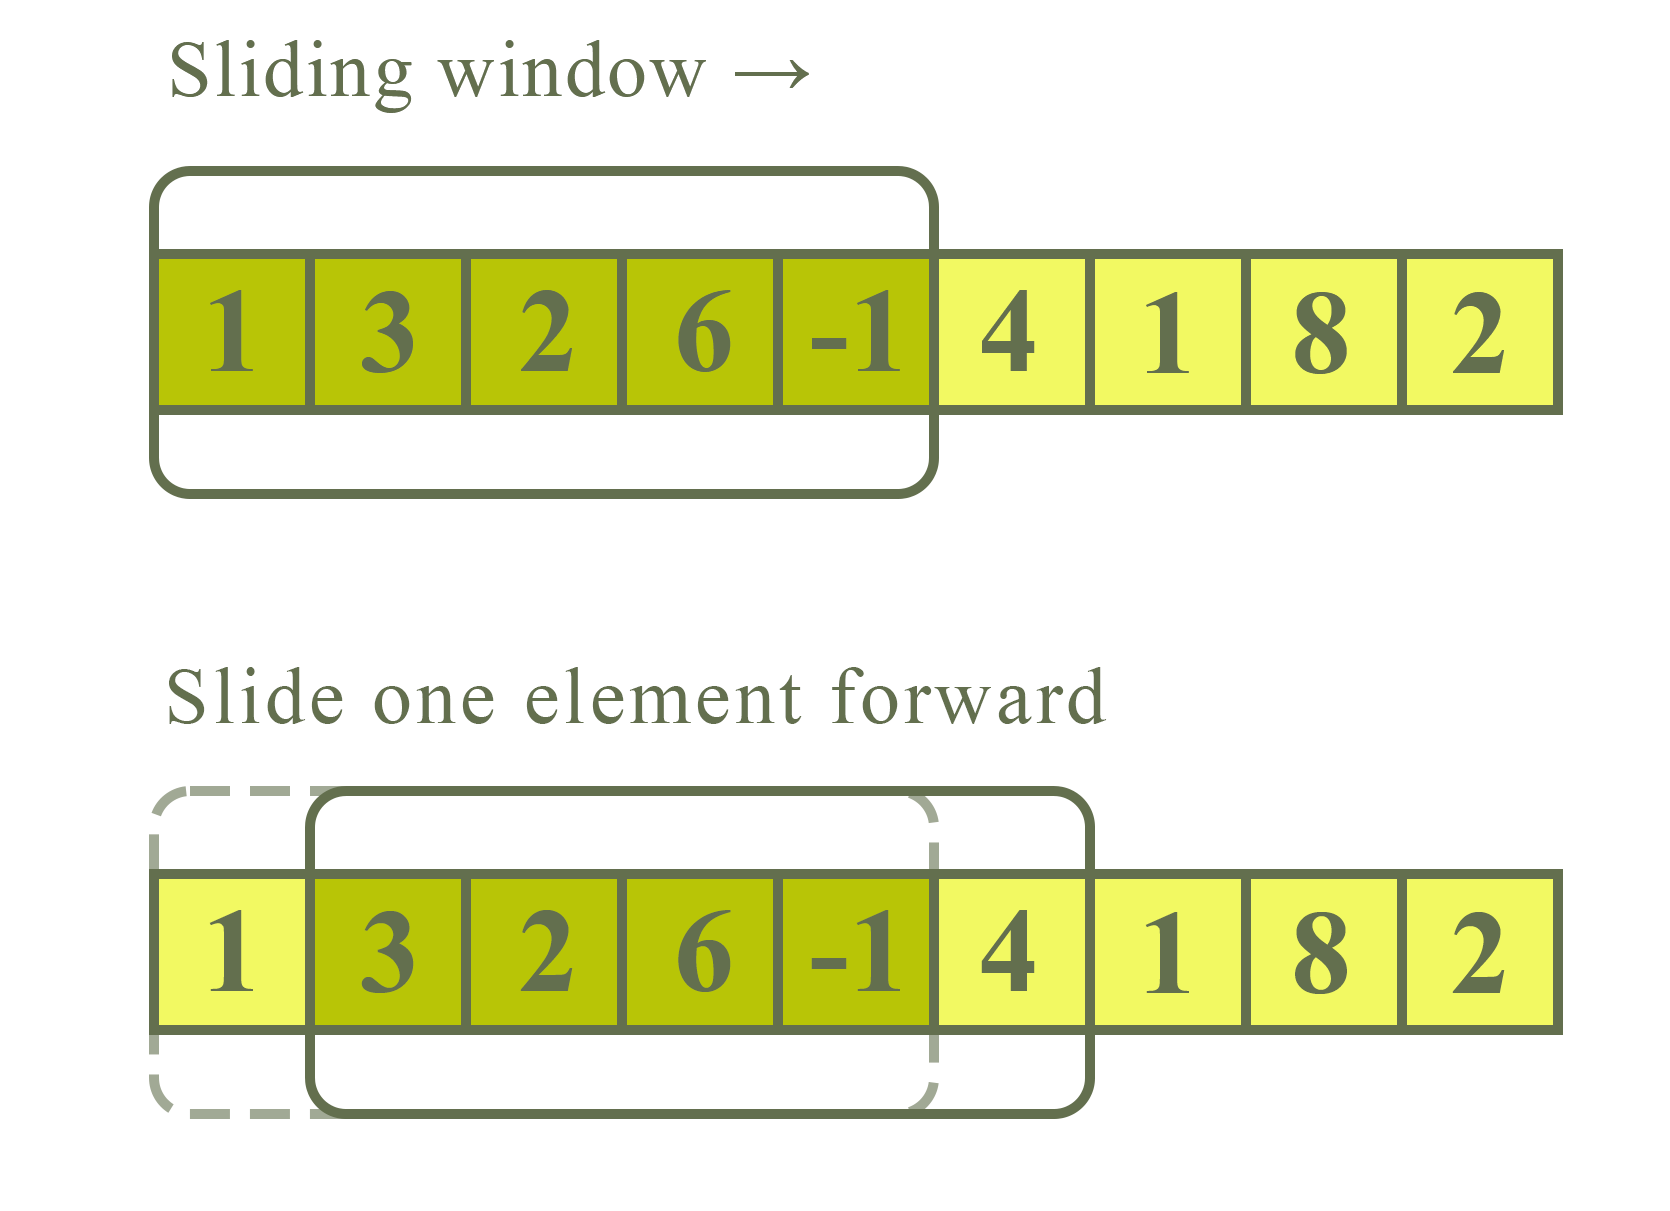
\includegraphics[width=12cm]{滑动窗口高清重制.png}
    \caption{Sketch of Sliding Window Algorithm} \label{Figure 18}
\end{figure}

We can briefly describe the process of the sliding window algorithm.
\begin{itemize}
    \item {\bf We start by initializing the parameters:}
    \item 
    Window size:W:10 (consider the last 10 scoring points)

    We notice that determining the sliding window size in units of 10 helps to fit the actual
    situation. It is possible to accurately measure the impact of the athlete's past performance on
    the present, but it is also possible to effectively control the size of the window to avoid the
    transitional impact of the past situation on the present, and to imply that the athlete will be
    positively adjusting his mindset for the following competitions. 

    Starting value of attenuation factor $D_{start}$:10

    attenuation step $D_{step}$:0.1

    \item {\bf For each score point, we perform the following steps:}
    \item[a.]{\bf Determine the sliding window}: Select a sliding window of W score points counting
    forward from the current score point i. If the current score point i is less than the previous
    score point, then take as many score points as possible. Take as many score points as possible
    if the previous score points are less than W.
    \item[b.]{\bf Calculating the attenuation weights:}For each score point j in the window, we calculate
    its decay weight $D_{j}$.$D_{j}$ refers to the magnitude of the momentum influencing factors decrease
    as the interval to the target time increases, also, the decreasing trend demonstrates a linear
    pattern, which in accordance with $D_{step}$. This notation is also in consistent with the actuality of what we feel in real life. The further back in time an event occurs, the less impact it will
    cause on the present. So the weight closest to the current score point is $D_{step}$, and for each score point moved forward, the weight decreases by $D_{step}$. At the same time, we guarantee
    that the minimum value of $D_{j}$ is $D_{step}$.

    \begin{equation} \label{15}
        D_{j}=D_{start}-(D_{step}\times(W-J))
    \end{equation}

    \item[c.]{\bf Weighted feature calculation:}For each score within the window, we calculate the
    weighted value of each feature $F_{k}$ and multiplied by the corresponding decay weight $D_{j}$,
    \begin{equation} \label{16}
        F^{'} _{k,j} =F _{k,j} \times D_{j}
    \end{equation}
    where$F^{'} _{k,j}$, is the weighted eigenvalue and $F_{k,j}$ is the original eigenvalue.
    \item[d.]{\bf Calculation of momentum indicators:} For each feature, the weighted eigenvalues of all
    the scores in the window are summed to obtain a momentum indicator for that feature $M_{k}$:
    \begin{equation} \label{17}
        M_{k}= {\textstyle \sum_{j=1}^{W}F^{'} _{k,j}} 
    \end{equation}
    Then, based on the feature importance weights$ M_{k}$, we calculate the weighted Momentum
    Indicator:
    \begin{equation} \label{18}
        M= {\textstyle \sum_{k=1}^{n}M_{k}\times M_{k}} 
    \end{equation}
    \item {\bf Momentum Indicator Updates and Model Training:}We train the model using the
    momentum indicator $M$ calculated in the above steps as one of the input features of the model. Additionally, we also adjust the sliding window size $W$, the decay factors $D_{start}$ and $D_{step}$ to
    optimize the model performance according to the model training results and performance
    evaluation needs.

\end{itemize}

 In conclusion, this algorithmic process utilizes the concept of time decay to give greater
weight to the most recent scoring points, allowing for more sensitive capture of immediate
changes in game momentum. With this approach, a dynamic predictive model can be
constructed that reflects changes in game momentum. 
Results are presented as follows:

\begin{figure}[htbp]
    \centering
    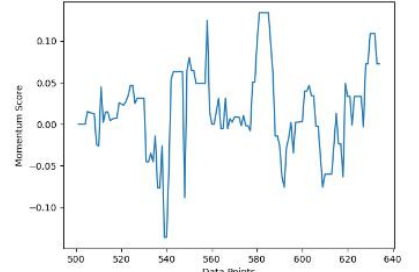
\includegraphics[width=8cm]{screencut 2025-01-22 163353.png}
    \caption{Momentum Score Over Time for 2023-wimbledon-1303} \label{Figure 19}
\end{figure}

According to the requirements of Problem 3, we need to prove the validity of the prediction
results of the new model we built to quantify momentum. We continue to use Logistic Regression
for predictive testing of the model's accuracy.

We note that unlike problem one, when we quantify momentum by directly using the characteristic elements, we can observe the result that most of the compared momentum value
integrals are positive, which implies that the previously built model may amplify the good
performance of a particular athlete while relatively ignoring the worse performance.

When we quantify the momentum values in Problem 3 by using the newly defined values of
the various ratios, we find that most of the compared momentum value integrals are negative, and
this will have a negative effect on our measurement of momentum. To avoid this problem, we
input $S_{p1i}$,$S_{p2i}$ separately instead of input $X_{i}$ as a ratio.

Next, we input ($S_{p1i}$,$S_{p2i}$,$Y_{i}$) as a sample set and train it, the results are presented in the
following graph:

\begin{figure}[htbp]
    \centering
    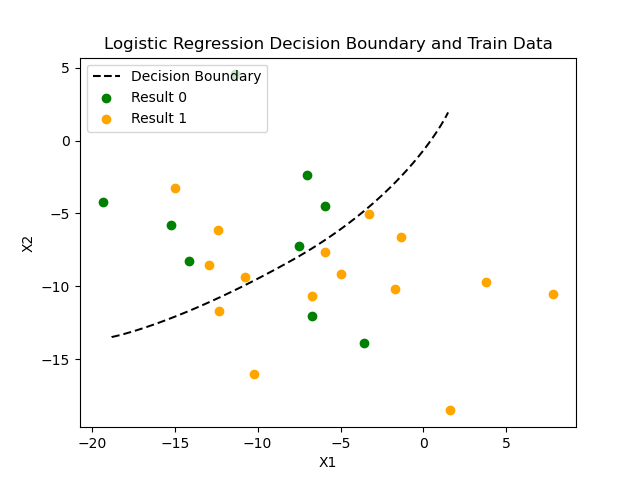
\includegraphics[width=12cm]{拟合1.png}
    \caption{Logistic Regression Decision Boundary} \label{Figure 20}
\end{figure}

Based on the above process, we can illustrate the validity of the model with full affirmation
of the correctness of the model's predictions.

\subsubsection{Identifying Turning Points in Swings}
Next, we are going to predict the swings in the match. Our research object shifts from
predictions on the outcome of the match to factors affecting momentum swings, in other words, our research perspective transferred from a holistic grasp to a partly and refined analysis of the
subject.\\
We continue to use the ratios from problem 1 and apply Random Forests to recreate a model. Firstly, we redefine $Y_{i}$. Different from the previous one, $Y_{i}$presented here refers to the turning
point in the trend fluctuation curve of the athlete's momentum value, where a value of 0 means
that the athlete's momentum has no turning point at this scoring point, and 1 means that the
athlete's momentum has turned at this scoring point. And $X_{i}$ is defined as before.

\begin{figure}[H]
    \centering
    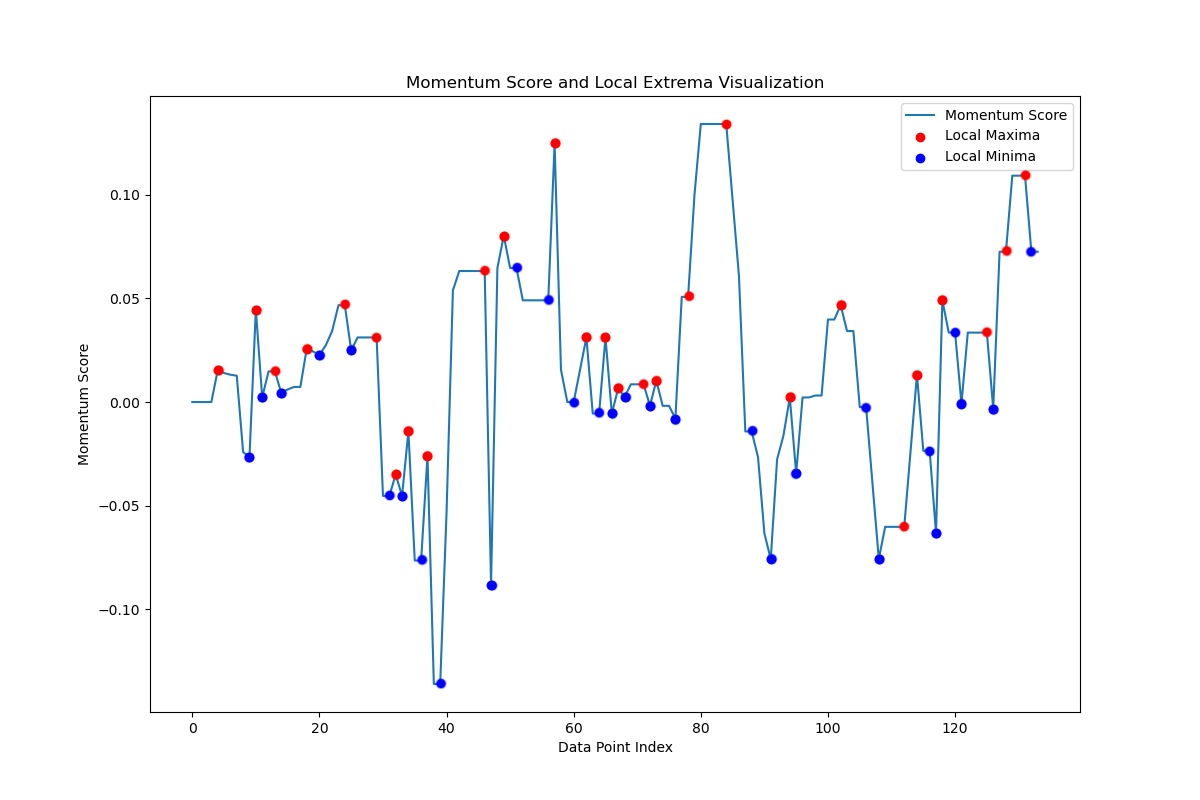
\includegraphics[width=8cm]{变化.png}
    \caption{Momentum Score and Local Extreme Visualization} \label{Figure 21}
\end{figure}

Then we determine the tendency of momentum and find the sequence of $Y_{i}$. We first locate
all the extreme points in the graph of the momentum value. We design a program to process the
curve, from which we found all the turning points in the curve and obtain the sequence of $Y_{i}$, which is
Y values: [0.0, 0.0, 1.0,1.0…]. Next we utilize sliding window algorithm to acquire the sequence of
$X_{i}$.In this way, we are able to produce the dataset ($X_{i}$,$Y_{i}$)and put it into the random forest to
generate a new set of weights for swings in momentum.

Results are listed in the diagram as follows:
\begin{table}[H]
    \centering
    \caption{\textbf{Feature Importance Ranking in Random Forest Model}}
    \vspace{-0.3pt}
    \begin{tabularx}{\textwidth}{>{\centering\arraybackslash}X>{\centering\arraybackslash}X>{\centering\arraybackslash}X}
    \toprule[2pt]
    \textbf{Order} & \textbf{Features}     & \textbf{Weights} \\ 
    \midrule[1pt]
    1              & break\_fail\_ratio    & 0.247522         \\ 
    2              & point\_victor         & 0.168837         \\ 
    3              & unf\_err              & 0.139420         \\ 
    4              & winner                & 0.108685         \\ 
    5              & ace                   & 0.095252         \\ 
    6              & double\_fault         & 0.077130         \\ 
    7              & net\_pt               & 0.074068         \\ 
    8              & net\_pt\_won          & 0.039238         \\ 
    9              & break\_pt\_missed     & 0.021428         \\ 
    \bottomrule[2pt]
    \end{tabularx}
    \label{tab:feature_importance}
    \end{table}

    \begin{figure}[H]
        \centering
        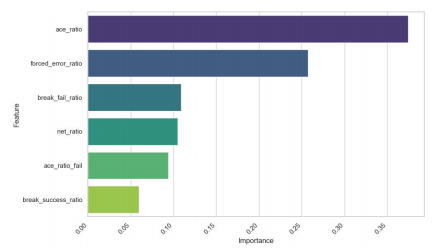
\includegraphics[width=8cm]{screencut 2025-01-22 164913.png}
        \caption{Factors Influencing Momentum Swings} \label{Figure 22}
    \end{figure}
    
    From the data in the graph, we can conclude that an unstoppable serve as the factor $A_{r}$
    , which
    refers to service score rate, with the largest weighting, i.e., as the element most associated with
    fluctuations in momentum changes, will have the potential to influence or even determine key
    changes or processes in a match. In the contrast, the factor $B_{r}$
    , which refers to break success rate, has a lower weight value, meaning that the athlete's momentum does not fluctuate greatly after
    winning a game. The reason to explain that result is that while $B_{r}$
    is important for overall match
    results, switching points to see that breaks don't matter in the middle. Another interesting finding
    is that the factor Fr, referring to the service failure rate, turns out to be insignificant in momentum
    fluctuation. This may be due to the fact that the athletes are prone to maintain a better state of    mind and believe in their own strengths in order to prepare themselves for the score later on.
    \subsubsection{Advices Towards a Different Player}
    Based on the weights of the factors we derived above, we can more accurately determine the
    changes in momentum fluctuations of the athletes in the course of the game, try to analyze the
    reasons for the changes in momentum fluctuations of the athletes, and provide suggestions for the
    game performance of the athletes during the match.
    \begin{itemize}
        \item {\bf A high level of self-confidence is a prerequisite for a victory:}As we can see from the
        results of the weighting, the percentage of serving points is in the first place of the weighting, which means that the confidence brought by successful serving points is the primary factor for
        athletes to keep their morale at a rather high level during the match. True self-confidence enables
        athletes to have a reasonable expectation of success, to actively and orderly deal with their game
        behavior, to think more quickly and rationally, and to have a clearer and more coordinated sense of
        technique, which lays the foundation for creating a good performance.
        \item {\bf Competitive strength and thorough preparation are the foundation for a victory:}We
        can tell that the change of the error ratio to the momentum fluctuation is still large. A good athlete
        should train actively to minimize the errors during the game, improve the technical level and
        tactical adjustment ability, so that he or she has a strong competitive strength and full preparation. Collecting opponents’ performance information during the season is also included in the
        preparations.
    
        \begin{figure}[htbp]
            \centering
            \subfloat[]{
            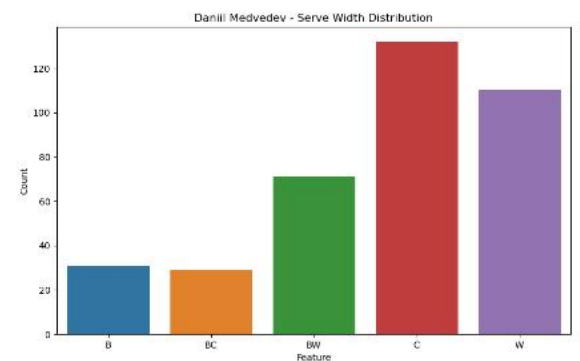
\includegraphics[width=6cm]{screencut 2025-01-22 165405.png}}
            \subfloat[]{
                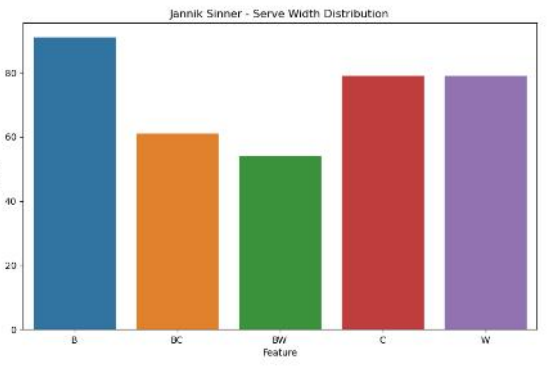
\includegraphics[width=6cm]{screencut 2025-01-22 165410.png}}
            \caption{Width of player's serve} \label{Figure 22-23}
        \end{figure}
    
        \item {\bf Be cautious consistently throughout the whole match is indispensable for a victory:}
        We
        know from the weight of the breaks that an exceptional athlete will remain cautious even when he
        or she is scoring points, not letting down the guard against the opponent, but continuing to play
        steadily and looking for opportunities to break through the opponent's defenses.\\
        \item {\bf Stress management also plays an important role for a victory:}The calculated weighting
        values indicate that the service failure rate also present a rather high value towards the swings of
        momentum. A brilliant athlete is supposed to perform even if they are faced with great pressure
        from opponents with fierce strength. It is necessary to face this pressure as a common feeling
        correctly and do well under pressure.
    \end{itemize}

    \subsection{Model Testing and Expansion}
According to the requirements of Problem 4, we want to further test the predictive power of
the model built previously. Unlike the previous one, here we artificially divide the time 80\% for
the training set and 20\% for the testing set, and the training results are shown as follows:

\begin{figure}[htbp]
    \centering
    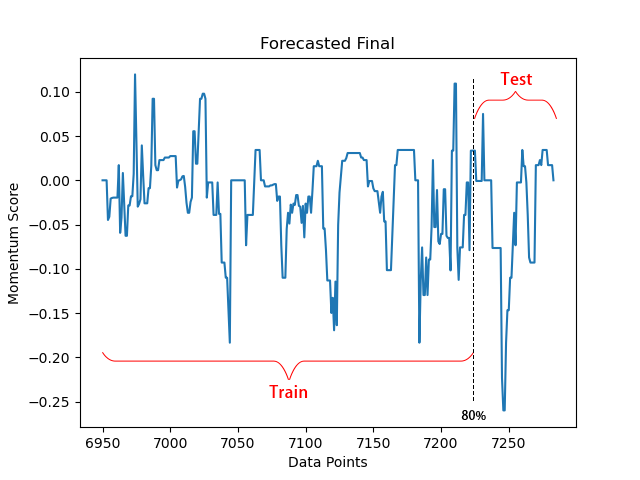
\includegraphics[width=12cm]{最终预测.png}
    \caption{Sketch of Segment} \label{Figure 24}
\end{figure}

Ultimately, we arrive at a model with 71\% predictive accuracy. It is rather high for predictive
modeling. Therefore its reliability can also be confirmed.

Next, we analyze further to figure out the expansion of the model in other conditions. If the
model performs poorly in certain situations, this may indicate that the model is missing some key
predictors or that the model is unable to capture all of the complex dynamics that affect the
momentum of the game. In response, we need to identify and supplement the possible missing
factors, and perform a series of more in-depth data analysis and adjustments to improve the
model's predictive power and generalizability.
\begin{itemize}
    \item {\bf Player Status:}Consider the player's physical condition, injury history, and mental state.
    \item {\bf Environmental factors:}e.g. weather conditions, location of the match, spectator support, etc.
    \item {\bf Historical performance:}a player's past match record, especially against specific
    opponents.
    \item {\bf Real-time data:}e.g. heart rate monitoring data during a match, which can provide
    information about a player's stress and fitness status.
    \item {\bf Style of Play:}Players' playing styles and strategies and how they affect the momentum of
    the game.
    \item {\bf Technical Statistics:}: more detailed technical statistics such as first serve success rate, net
    scoring rate, unforced errors, etc.
    \item {\bf Stress coping:}a player's ability to manage stress at critical moments.
    \item {\bf Dynamic mental states:}players' confidence and motivation levels during the game.
\end{itemize}

For women's tournaments, the model may need to analyze the data to identify the different
characteristics of momentum changes in men's and women's tournaments. For tournaments, their
level and type may affect player performance and the model needs to be able to accommodate
these differences. For different court surfaces (hardcourt, grass, red clay) affecting ball bounce and
speed of play, this needs to be captured in the model. For other sports, such as table tennis, the
model needs to be adapted to match different scoring systems and pace of play.

Through the above process, we can identify key factors that may be missing from the current
model and propose targeted improvements. At the same time, we can also assess the model's
ability to generalize under different conditions and adjust the model accordingly to fit different
playing environments and rules. This iterative process will help build stronger and more accurate
predictive models, and ultimately provide more valuable strategic advice to coaches and players!
%%%%%%%%%%%%%%%%%%%%%%%%%%%%%%%%%%%%%%%敏感性分析%%%%%%%%%%%%%%%%%%%%%%%%%%%%%%%%%%%%%%%%
\section{Sensitivity Analysis}
In the sensitivity analysis of the momentum prediction model for the 2023 Wimbledon tennis
tournament, we explored the impact of different sliding window sizes (8, 10, 15) on the model's
accuracy and the importance of its features. The charts illustrate the variation in momentum scores
over time for each of the three different window sizes, as well as the corresponding importance of
feature scores.
\begin{figure}[htbp]
    \centering
    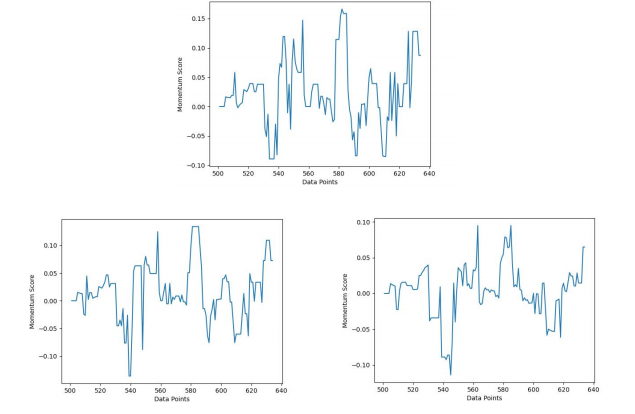
\includegraphics[width=12cm]{screencut 2025-01-22 170236.png}
    \caption{Momentum scores at different sizes} \label{Figure 25}
\end{figure}

\begin{table}[H]
    \centering
    \caption{\textbf{Feature Importance Ranking in Random Forest Model}}
    \vspace{-0.3pt}
    \begin{threeparttable}
    \begin{tabularx}{\textwidth}{>{\centering\arraybackslash}X>{\centering\arraybackslash}X>{\centering\arraybackslash}X}
    \toprule[2pt]
    \textbf{Order} & \textbf{Features}     & \textbf{Weights} \\ 
    \midrule[1pt]
    1              & break\_fail\_ratio    & 0.247522         \\ 
    2              & point\_victor         & 0.168837         \\ 
    3              & unf\_err              & 0.139420         \\ 
    4              & winner                & 0.108685         \\ 
    5              & ace                   & 0.095252         \\ 
    6              & double\_fault         & 0.077130         \\ 
    7              & net\_pt               & 0.074068         \\ 
    8              & net\_pt\_won          & 0.039238         \\ 
    9              & break\_pt\_missed     & 0.021428         \\ 
    \bottomrule[2pt]
    \end{tabularx}
    \label{tab:feature_importance}
    \begin{tablenotes}
        \footnotesize
        \item Model Accuracy: 0.5925925925925926
      \end{tablenotes}
    \end{threeparttable}
    \end{table}

    \begin{table}[H]
        \centering
        \caption{\textbf{Feature Importance Ranking in Random Forest Model}}
        \vspace{-0.3pt}
        \begin{threeparttable}
        \begin{tabularx}{\textwidth}{>{\centering\arraybackslash}X>{\centering\arraybackslash}X>{\centering\arraybackslash}X}
        \toprule[2pt]
        \textbf{Order} & \textbf{Features}     & \textbf{Weights} \\ 
        \midrule[1pt]
        1              & break\_fail\_ratio    & 0.247522         \\ 
        2              & point\_victor         & 0.168837         \\ 
        3              & unf\_err              & 0.139420         \\ 
        4              & winner                & 0.108685         \\ 
        5              & ace                   & 0.095252         \\ 
        6              & double\_fault         & 0.077130         \\ 
        7              & net\_pt               & 0.074068         \\ 
        8              & net\_pt\_won          & 0.039238         \\ 
        9              & break\_pt\_missed     & 0.021428         \\ 
        \bottomrule[2pt]
        \end{tabularx}
        \label{tab:feature_importance}
        \begin{tablenotes}
            \footnotesize
            \item Model Accuracy: 0.7777777777777778
          \end{tablenotes}
        \end{threeparttable}
        \end{table}
        

        With a window size of 8, the model accuracy was 59.26\%, suggesting that the model may not
capture enough information within shorter time windows to accurately predict momentum shifts. The ranking of feature importance shows that the ace\_ratio (ace scoring rate) has the highest
weight of 0.353956, indicating that it is a key factor in influencing model predictions even within
a shorter timeframe.

As the window size increases to 10, we observe a significant improvement in accuracy, and
the distribution of feature importance shifts as well. At a window size of 15, the accuracy of the
model slightly decreases to 70.37\%, possibly because the longer time window includes too much
information, diluting the impact of some key short-term changes.

Across all window sizes, the ace\_ratio remains the most important feature, especially at a
window size of 15, where its weight increases to 48.73\%, further emphasizing the importance of
the ace scoring rate in predicting momentum changes. The forced\_error\_ratio (forced error rate)
maintains high importance across all window sizes, particularly at window sizes of 8 and 15, suggesting that forced errors are a consistent factor affecting the momentum shifts in matches.

When selecting a window size, it is necessary to balance changes in accuracy and feature
importance to find the optimal window size that enhances the predictive performance of the model. As the charts suggest, a moderate window size (such as 10) appears to provide the best balance
between accuracy and the importance of features.
\end{document}

